\documentclass[border=4pt]{standalone}
% Shared typography and colours for the standalone figures.
\usepackage{unicode-math}
\setmainfont{TeX Gyre Termes}
\setmathfont{TeX Gyre Termes Math}
\usepackage{tikz}
\usetikzlibrary{arrows.meta,positioning,calc,decorations.pathreplacing}
\usepackage{pgfplots}
\pgfplotsset{compat=1.18}

% One colour per element or subsystem. Record the mapping in
% the working repository conventions and use it identically in every figure.
\definecolor{elemA}{HTML}{1F5FA8}
\definecolor{elemB}{HTML}{B8461B}
\definecolor{elemC}{HTML}{2E7D32}
\definecolor{elemD}{HTML}{6A4C93}
\definecolor{frameline}{HTML}{555555}

\usetikzlibrary{decorations.pathmorphing}
\begin{document}
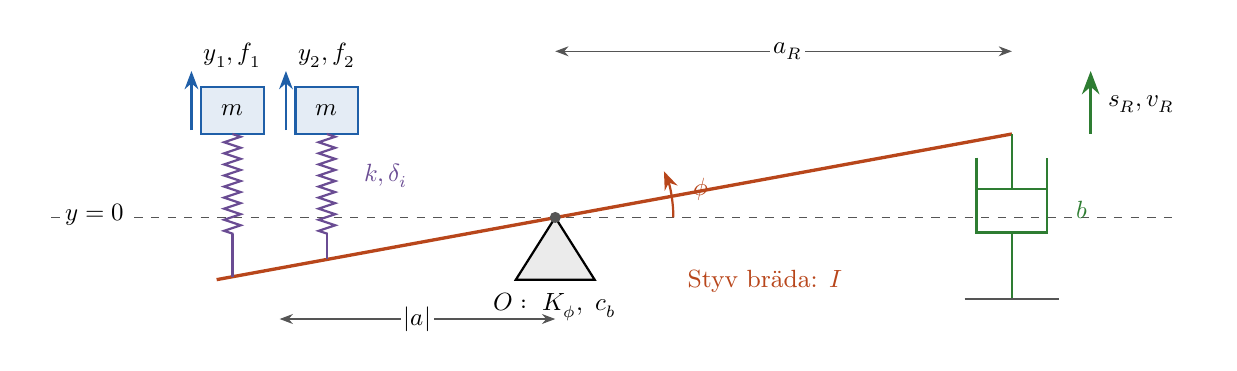
\begin{tikzpicture}[>=Stealth,font=\small]
\path[use as bounding box] (0,-.9) rectangle (15,3.1);
\draw[dashed,frameline] (.3,.69)--(14.6,.69);
\node[anchor=west,fill=white,inner sep=2pt] at (.4,.72) {$y=0$};
\draw[very thick,elemB] (2.4,-.1)--(12.5,1.75);
\draw[fill=frameline!12,thick] (6.7,.69)--(6.2,-.1)--(7.2,-.1)--cycle;
\fill[frameline] (6.7,.69) circle (2pt);
\node[below] at (6.7,-.15) {$O:\ K_\phi,\ c_b$};
\draw[->,elemB,thick] (8.2,.69) arc (0:23:1.5);
\node[elemB] at (8.55,1.05) {$\phi$};
\foreach \x/\lab in {2.6/1,3.8/2}{
 \draw[fill=elemA!12,draw=elemA,thick] (\x-.4,1.75) rectangle (\x+.4,2.35);
 \node at (\x,2.05) {$m$};
 \draw[decorate,decoration={zigzag,segment length=4pt,amplitude=3pt},elemD,thick] (\x,1.75)--(\x,.48);
 \draw[elemD,thick] (\x,.48)--(\x,{-.1+(\x-2.4)*1.85/10.1});
 \draw[->,elemA,thick] (\x-.52,1.8)--(\x-.52,2.55);
 \node at (\x,2.75) {$y_{\lab},f_{\lab}$};
}
\node[elemD] at (4.55,1.22) {$k,\delta_i$};
\draw[<->,frameline] (3.2,-.6)--(6.7,-.6);
\node[fill=white,inner sep=1pt] at (4.95,-.6) {$|a|$};
\draw[<->,frameline] (6.7,2.8)--(12.5,2.8);
\node[fill=white,inner sep=1pt] at (9.65,2.8) {$a_R$};
\draw[elemC,thick] (12.5,1.75)--(12.5,1.05);
\draw[elemC,thick] (12.05,1.05)--(12.95,1.05);
\draw[elemC,thick] (12.05,1.45)--(12.05,.5)--(12.95,.5)--(12.95,1.45);
\draw[elemC,thick] (12.5,.5)--(12.5,-.35);
\draw[frameline,thick] (11.9,-.35)--(13.1,-.35);
\draw[->,elemC,very thick] (13.5,1.75)--(13.5,2.55);
\node[anchor=west] at (13.6,2.13) {$s_R,v_R$};
\node[anchor=west,elemC] at (13.2,.78) {$b$};
\node[elemB] at (9.35,-.12) {Styv bräda: $I$};
\end{tikzpicture}
\end{document}
